%
% Template Laporan Skripsi/Thesis 
%
% @author  Andreas Febrian, Lia Sadita 
% @version 1.03
%
% Dokumen ini dibuat berdasarkan standar IEEE dalam membuat class untuk 
% LaTeX dan konfigurasi LaTeX yang digunakan Fahrurrozi Rahman ketika 
% membuat laporan skripsi. Konfigurasi yang lama telah disesuaikan dengan 
% aturan penulisan thesis yang dikeluarkan UI pada tahun 2008.
%

%
% Tipe dokumen adalah report dengan satu kolom. 
%
\documentclass[12pt, a4paper, onecolumn, oneside, final]{report}

% Load konfigurasi LaTeX untuk tipe laporan thesis
\usepackage{uithesis}


% Load konfigurasi khusus untuk laporan yang sedang dibuat
%-----------------------------------------------------------------------------%
% Informasi Mengenai Dokumen
%-----------------------------------------------------------------------------%
% 
% Judul laporan. 
\var{\judul}{Open Domain Information Extraction Otomatis dari Teks Bahasa Indonesia}
% 
% Tulis kembali judul laporan, kali ini akan diubah menjadi huruf kapital
\Var{\Judul}{Open Domain Information Extraction Otomatis dari Teks Bahasa Indonesia}
% 
% Tulis kembali judul laporan namun dengan bahasa Ingris
\var{\judulInggris}{Automatic Open Domain Information Extraction from Indonesian Text}

% 
% Tipe laporan, dapat berisi Skripsi, Tugas Akhir, Thesis, atau Disertasi
\var{\type}{Tesis}
% 
% Tulis kembali tipe laporan, kali ini akan diubah menjadi huruf kapital
\Var{\Type}{Tesis}
% 
% Tulis nama penulis 
\var{\penulis}{Yohanes Gultom}
% 
% Tulis kembali nama penulis, kali ini akan diubah menjadi huruf kapital
\Var{\Penulis}{Yohanes Gultom}
% 
% Tulis NPM penulis
\var{\npm}{1506706345}
% 
% Tuliskan Fakultas dimana penulis berada
\Var{\Fakultas}{Ilmu Komputer}
\var{\fakultas}{Ilmu Komputer}
% 
% Tuliskan Program Studi yang diambil penulis
\Var{\Program}{Magister Ilmu Komputer}
\var{\program}{Magister Ilmu Komputer}
% 
% Tuliskan tahun publikasi laporan
\Var{\bulanTahun}{Juni 2017}
% 
% Tuliskan gelar yang akan diperoleh dengan menyerahkan laporan ini
\var{\gelar}{Magister Ilmu Komputer}
% 
% Tuliskan tanggal pengesahan laporan, waktu dimana laporan diserahkan ke 
% penguji/sekretariat
\var{\tanggalPengesahan}{6 Juni 2017} 
% 
% Tuliskan tanggal keputusan sidang dikeluarkan dan penulis dinyatakan 
% lulus/tidak lulus
\var{\tanggalLulus}{6 Juni 2017}
% 
% Tuliskan pembimbing 
\var{\pembimbing}{Wahyu Catur Wibowo, Ir., M.Sc., Ph.D.}
% 
% Alias untuk memudahkan alur penulisan paa saat menulis laporan
\var{\saya}{Penulis}

%-----------------------------------------------------------------------------%
% Judul Setiap Bab
%-----------------------------------------------------------------------------%
% 
% Berikut ada judul-judul setiap bab. 
% Silahkan diubah sesuai dengan kebutuhan. 
% 
\Var{\kataPengantar}{Kata Pengantar}
\Var{\babSatu}{Pendahuluan}
\Var{\babDua}{Landasan Teori}
\Var{\babTiga}{Metode Penelitian}
\Var{\babEmpat}{Hasil dan Analisis}
\Var{\babLima}{Penutup}

% Daftar pemenggalan suku kata dan istilah dalam LaTeX
%
% Hyphenation untuk Indonesia 
%
% @author  Andreas Febrian
% @version 1.00
% 
% Tambahkan cara pemenggalan kata-kata yang salah dipenggal secara otomatis 
% oleh LaTeX. Jika kata tersebut dapat dipenggal dengan benar, maka tidak 
% perlu ditambahkan dalam berkas ini. Tanda pemenggalan kata menggunakan 
% tanda '-'; contoh:
% menarik
%   --> pemenggalan: me-na-rik
%

\hyphenation{
    % alphabhet A
    a-na-li-sa a-tur 
    a-pli-ka-si 
    % alphabhet B
    ba-ngun-an 
    be-be-ra-pa 
    ber-ge-rak
    ber-ke-lan-jut-an 
    ber-pe-nga-ruh 
    % alphabhet C
    ca-ri
    % alphabhet D
    di-sim-pan di-pim-pin de-ngan da-e-rah di-ba-ngun da-pat di-nya-ta-kan 
    di-sim-bol-kan di-pi-lih di-li-hat de-fi-ni-si di-pi-sah-kan
    % alphabhet E
    e-ner-gi eks-klu-sif
    % alphabhet F
    fa-si-li-tas
    % alphabhet G
    ga-bung-an ge-rak
    % alphabhet H
    ha-lang-an
    % alphabhet I
    % alphabhet J
    % alphabhet K
    ke-hi-lang-an
    ku-ning 
    kua-li-tas ka-me-ra ke-mung-kin-an ke-se-pa-ham-an
    % alphabhet L
    ling-kung-an
    % alphabhet M
    me-neng-ah
    meng-a-tas-i me-mung-kin-kan me-nge-na-i me-ngi-rim-kan 
    meng-u-bah meng-a-dap-ta-si me-nya-ta-kan mo-di-fi-ka-si
    meng-a-tur
    % alphabhet N
    nya-ta non-eks-klu-sif
    % alphabhet O
    % alphabhet P
	pe-nye-rap-an 
	pe-ngon-trol
    pe-mo-del-an
    pe-ran  pe-ran-an-nya
    pem-ba-ngun-an pre-si-den pe-me-rin-tah prio-ri-tas peng-am-bil-an 
    peng-ga-bung-an pe-nga-was-an pe-ngem-bang-an 
    pe-nga-ruh pa-ra-lel-is-me per-hi-tung-an per-ma-sa-lah-an 
    pen-ca-ri-an peng-struk-tur-an
    % alphabhet Q
    % alphabhet R
    ran-cang-an
    % alphabhet S
    si-mu-la-si sa-ngat
    % alphabhet T
    te-ngah
    ter-da-pat
    % alphabhet U
    % alphabhet V
    % alphabhet W
    % alphabhet X
    % alphabhet Y
    % alphabhet Z
    % special
}
% Daftar istilah yang mungkin perlu ditandai 
%
% @author  Andreas Febrian
% @version 1.00
% 
% Mendaftar seluruh istilah yang mungkin akan perlu dijadikan 
% italic atau bold pada setiap kemunculannya dalam dokumen. 
% 

\var{\license}{\f{Creative Common License 1.0 Generic}}
\var{\bslash}{$\setminus$}

% Awal bagian penulisan laporan
\begin{document}
%
% Sampul Laporan
%
% Sampul Laporan

%
% @author  unknown
% @version 1.01
% @edit by Andreas Febrian
%

\begin{titlepage}
    \begin{center}    
        \begin{figure}
            \begin{center}
                
\includegraphics[width=2.5cm]{pics/makara.png}
            \end{center}
        \end{figure}    
        \vspace*{0cm}
        \bo{
        	UNIVERSITAS INDONESIA\\
        }
        
        \vspace*{1.0cm}
        % judul thesis harus dalam 14pt Times New Roman
        \bo{\Judul} \\[1.0cm]

        \vspace*{2.5 cm}    
        % harus dalam 14pt Times New Roman
        \bo{\Type}

        \vspace*{3 cm}       
        % penulis dan npm
        \bo{\Penulis} \\
        \bo{\npm} \\

        \vspace*{5.0cm}

        % informasi mengenai fakultas dan program studi
        \bo{
        	FAKULTAS \Fakultas\\
        	PROGRAM STUDI \Program \\
        	DEPOK \\
        	\bulanTahun
        }
    \end{center}
\end{titlepage}


%
% Gunakan penomeran romawi
\pagenumbering{roman}

%
% load halaman judul dalam
\addChapter{HALAMAN JUDUL}
%
% Halaman Judul Laporan 
%
% @author  unknown
% @version 1.01
% @edit by Andreas Febrian
%

\begin{titlepage}
    \begin{center}\begin{figure}
            \begin{center}
                
\includegraphics[width=2.5cm]{pics/makara.png}
            \end{center}
        \end{figure}    
        \vspace*{0cm}
        \bo{
        	UNIVERSITAS INDONESIA\\
        }
        
        \vspace*{1.0cm}
        % judul thesis harus dalam 14pt Times New Roman
        \bo{\Judul} \\[1.0cm]

        \vspace*{2.5 cm}    
        % harus dalam 14pt Times New Roman
        \bo{\Type} \\
        % keterangan prasyarat
        \bo{Diajukan sebagai salah satu syarat untuk memperoleh gelar \\
        \gelar}\\

        \vspace*{3 cm}       
        % penulis dan npm
        \bo{\Penulis} \\
        \bo{\npm} \\

        \vspace*{5.0cm}

        % informasi mengenai fakultas dan program studi
        \bo{
        	FAKULTAS \Fakultas\\
        	PROGRAM STUDI \Program \\
        	DEPOK \\
        	\bulanTahun
        }
    \end{center}
\end{titlepage}

%
% setelah bagian ini, halaman dihitung sebagai halaman ke 2
\setcounter{page}{2}


% load halaman pengesahan
\addChapter{LEMBAR PERSETUJUAN}
%
% Halaman Pengesahan
%
% @author  Andreas Febrian
% @version 1.01
%

\chapter*{HALAMAN PERSETUJUAN}

\vspace*{0.2cm}
\noindent 

\noindent
\begin{tabular}{l l p{11cm}}
	\bo{Judul}&: & \judul \\ 
	\bo{Nama}&: & \penulis \\
	\bo{NPM}&: & \npm \\
\end{tabular} \\

\vspace*{1.2cm}

\noindent Laporan \type~ini telah diperiksa dan disetujui.\\[0.3cm]
\begin{center}
\tanggalPengesahan \\[2cm]


\underline{\pembimbing}\\[0.1cm]
Pembimbing \type
\end{center}

\newpage

% load halaman orisinalitas 
\addChapter{LEMBAR PERNYATAAN ORISINALITAS}
%
% Halaman Orisinalitas
%
% @author  Andreas Febrian
% @version 1.01
%

\chapter*{\uppercase{halaman pernyataan orisinalitas}}
\vspace*{2cm}

\begin{center}
	\bo{\type~ini adalah hasil karya saya sendiri, \\ 
	dan semua sumber baik yang dikutip maupun dirujuk \\
	telah saya nyatakan dengan benar.} \\
	\vspace*{2.6cm}
	
	\begin{tabular}{l c l}
	\bo{Nama} & : & \bo{\penulis} \\
	\bo{NPM} & : & \bo{\npm} \\ 
	\bo{Tanda Tangan} & : & \\
	& & \\
	& & \\
	\bo{Tanggal} & : & \bo{\tanggalPengesahan} \\	
	\end{tabular}
\end{center}

\newpage


%\addChapter{LEMBAR PENGESAHAN}
%%
% Halaman Pengesahan Sidang
%
% @author  Andreas Febrian, Andre Tampubolon 
% @version 1.02
%

\chapter*{HALAMAN PENGESAHAN}

\vspace*{0.4cm}
\noindent 

\noindent
\begin{tabular}{ll p{9cm}}
	\type~ini diajukan oleh&: & \\
	Nama&: & \penulis \\
	NPM&: & \npm \\
	Program Studi&: & \program \\
	Judul \type&: & \judul \\
\end{tabular} \\

\vspace*{1.0cm}

\noindent \bo{Telah berhasil dipertahankan di hadapan Dewan Penguji 
dan diterima sebagai bagian persyaratan yang diperlukan untuk 
memperoleh gelar \gelar~pada Program Studi \program, Fakultas 
\fakultas, Universitas Indonesia.}\\[0.2cm]

\begin{center}
	\bo{DEWAN PENGUJI}
\end{center}

\vspace*{0.3cm}

\begin{tabular}{l l l l }
	& & & \\
	Pembimbing&: & \pembimbing & (\hspace*{3.0cm}) \\
	& & & \\
	Penguji&: & Prof. XXX & (\hspace*{3.0cm}) \\
	& & & \\
	Penguji&: & Prof. XXXX & (\hspace*{3.0cm}) \\
	& & & \\
	Penguji&: & Prof. XXXXXX & (\hspace*{3.0cm}) \\
\end{tabular}\\

\todo{Jangan lupa mengisi nama para penguji.}

\vspace*{2.0cm}

\begin{tabular}{ll l}
	Ditetapkan di&: & Depok\\
	Tanggal&: & \tanggalLulus \\
\end{tabular}


\newpage
%
%
%\addChapter{\kataPengantar}
%%-----------------------------------------------------------------------------%
\chapter*{\kataPengantar}
%-----------------------------------------------------------------------------%

Puji syukur saya panjatkan kepada Tuhan Yang Maha Esa, karena atas berkat dan rahmat-Nya, saya dapat menyelesaikan tesis ini. Penulisan tesis ini dilakukan dalam rangka memenuhi salah satu syarat untuk mencapai gelar Magister Ilmu Komputer pada Fakultas Ilmu Komputer Universitas Indonesia. Saya menyadari bahwa, tanpa bantuan dan bimbingan dari berbagai pihak, dari masa perkuliahan sampai pada penyusunan tesis ini, sangatlah sulit bagi saya untuk menyelesaikan tesis ini. Oleh karena itu, saya mengucapkan terima kasih kepada:

\begin{enumerate}
	\item Ir. Wahyu Catur Wibowo M.Sc., Ph.D., selaku dosen pembimbing yang telah menyediakan waktu, tenaga, dan pikiran untuk mengarahkan saya dalam penyusunan tesis ini;
	\item Rahmad Mahendra S.Kom., M.Sc., selaku dosen mata kuliah NLP yang memberikan banyak saran, kritik dan arahan teknis dalam melakukan penelitian tesis ini;
	\item ibu, adik-adik dan keluarga besar yang telah memberikan bantuan dukungan doa, moral dan material; serta
	\item rekan-rekan seperjuangan MIK 2015 yang namanya tidak dapat saya sebutkan satu per satu, yang telah banyak membantu saya dalam menyelesaikan tesis ini.
\end{enumerate}

Akhir kata, saya berharap Tuhan Yang Maha Esa berkenan membalas segala kebaikan semua pihak yang telah membantu. Semoga tesis ini membawa manfaat bagi pengembangan ilmu.

\vspace*{0.1cm}
\begin{flushright}
Depok, \tanggalPengesahan\\[0.1cm]
\vspace*{1cm}
\penulis

\end{flushright}
%
%
%\addChapter{LEMBAR PERSETUJUAN PUBLIKASI ILMIAH}
%% 
% @author  Andre Tampubolon, Andreas Febrian
% @version 1.01
% 

\chapter*{\uppercase{Halaman Pernyataan Persetujuan Publikasi Tugas Akhir untuk Kepentingan Akademis}}

\vspace*{0.2cm}
\noindent 
Sebagai sivitas akademik Universitas Indonesia, saya yang bertanda 
tangan di bawah ini:
\vspace*{0.4cm}


\begin{tabular}{p{4.2cm} l p{6cm}}
	\bo{Nama} & : & \penulis \\ 	
	\bo{NPM} & : & \npm \\
	\bo{Program Studi} & : & \program\\	
	\bo{Fakultas} & : & \fakultas\\
	\bo{Jenis Karya} & : & \type \\
\end{tabular}

\vspace*{0.6cm}
\noindent demi pengembangan ilmu pengetahuan, menyetujui untuk memberikan 
kepada Universitas Indonesia \bo{Hak Bebas Royalti Noneksklusif 
(Non-exclusive Royalty Free Right)} atas karya ilmiah saya yang berjudul:
\begin{center}
	\judul
\end{center}
beserta perangkat yang ada (jika diperlukan). Dengan Hak Bebas Royalti 
Noneksklusif ini Universitas Indonesia berhak menyimpan, 
mengalihmedia/formatkan, mengelola dalam bentuk pangkalan data 
(database), merawat, dan memublikasikan tugas akhir saya selama 
tetap mencantumkan nama saya sebagai penulis/pencipta dan sebagai 
pemilik Hak Cipta. \\

\noindent Demikian pernyatan ini saya buat dengan sebenarnya.

\begin{center}
	\vspace*{0.8cm}
	\begin{tabular}{lll}
		Dibuat di&: & Depok \\
		Pada tanggal&: & \tanggalPengesahan \\
	\end{tabular}\\

	\vspace*{0.2cm}
	Yang menyatakan \\
	\vspace*{1.1cm}
	(\penulis)
\end{center}

\newpage


%
% 
\addChapter{ABSTRAK}
%
% Halaman Abstrak
%
% @author  Andreas Febrian
% @version 1.00
%

\chapter*{Abstrak}

\vspace*{0.2cm}

\noindent \begin{tabular}{l l p{10cm}}
	Nama&: & \penulis \\
	Program Studi&: & \program \\
	Judul&: & \judul \\
\end{tabular} \\ 

\vspace*{0.5cm}

\noindent Banyaknya jumlah dokumen digital yang tersedia saat ini sudah melebihi kapasitas manusia untuk memprosesnya secara manual. Hal ini mendorong munculnya kebutuhan akan metode ekstrasi informasi (\textit{information extraction}) otomatis dari teks atau dokumen digital dari berbagai domain (\textit{open domain}). Sayangnya, sistem \textit{open domain information extraction} (\textit{open IE}) yang ada saat ini hanya berlaku untuk bahasa tertentu saja. Selain itu belum ada sistem \textit{open IE} untuk bahasa Indonesia yang dipublikasikan. Pada penelitian ini \saya memperkenalkan sebuah sistem untuk mengekstraksi relasi antar entitas dari teks bahasa Indonesia dari berbagai domain. Sistem ini menggunakan pembangkit kandidat \textit{triple} (\textit{triple candidates generator}) dan pengembang token (\textit{token expander}) berbasis aturan serta pemilih \textit{triple} berbasis \textit{machine learning}. Setelah melakukan \textit{cross-validation} terhadap empat kandidat model: \textit{logistic regression}, SVM, MLP dan \textit{Random Forest}, \saya menemukan bahwa \textit{Random Forest} adalah \textit{classifier} yang terbaik untuk dijadikan \textit{triple selector} denan skor F1 0.58 (\textit{precision} 0.62 dan \textit{recall} 0.58). Penyebab utama skor yang masih rendah ini adalah aturan pembangkitan kandidat yang masih sederhana dan cakupan pola \textit{dataset} yang masih rendah. \\

\vspace*{0.2cm}

\noindent Kata Kunci: \\ 
\noindent information extraction, open domain, natural language processing, bahasa Indonesia \\

\newpage
%
%
%
% Halaman Abstract
%
% @author  Andreas Febrian
% @version 1.00
%

\chapter*{ABSTRACT}

\vspace*{0.2cm}

\noindent \begin{tabular}{l l p{11.0cm}}
	Name&: & \penulis \\
	Program&: & \program \\
	Title&: & \judulInggris \\
\end{tabular} \\ 

\vspace*{0.5cm}

\noindent The vast amount of digital documents, that have surpassed human processing capability, calls for an automatic information extraction method from any text document regardless of their domain. Unfortunately, open domain information extraction (open IE) systems are language-specific and there is no published system for Indonesian language. This paper introduces a system to extract entity relations from Indonesian text in triple format using an NLP pipeline, rule-based candidates generator, token expander and supervised-learning-based triple selector. We cross-validate four candidates: logistic regression, SVM, MLP, Random Forest using our dataset to discover that Random Forest is the best classifier for the triple selector achieving 0.58 F1 score (0.62 precision and 0.58 recall). The low score is largely due to the simplistic candidate generation rules and the low quality of dataset. Overall the system is able to extract information efficiently from Indonesian text. However, the precision of the system is still very low due to the low performance of NLP pipeline and some limitations in token expander. \\

\vspace*{0.2cm}

\noindent Keywords: \\ 
\noindent information extraction, open domain, natural language processing, supervised learning, Indonesian language

\newpage

%
% Daftar isi, gambar, dan tabel
%
\tableofcontents
\clearpage
\listoffigures
\clearpage
\listoftables
\clearpage

%
% Gunakan penomeran Arab (1, 2, 3, ...) setelah bagian ini.
%
\pagenumbering{arabic}

%
%
%
%-----------------------------------------------------------------------------%
\chapter{\babSatu}
%-----------------------------------------------------------------------------%
\todo{tambahkan kata-kata pengantar bab 1 disini}


%-----------------------------------------------------------------------------%
\section{Latar Belakang}
%-----------------------------------------------------------------------------%
\todo{tuliskan latar belakang penelitian disini}


%-----------------------------------------------------------------------------%
\section{Permasalahan}
%-----------------------------------------------------------------------------%
Pada bagian ini akan dijelaskan mengenai definisi permasalahan 
yang \saya~hadapi dan ingin diselesaikan serta asumsi dan batasan 
yang digunakan dalam menyelesaikannya.


%-----------------------------------------------------------------------------%
\subsection{Definisi Permasalahan}
%-----------------------------------------------------------------------------%
\todo{Tuliskan permasalahan yang ingin diselesaikan. Bisa juga
	berbentuk pertanyaan}


%-----------------------------------------------------------------------------%
\subsection{Batasan Permasalahan}
%-----------------------------------------------------------------------------%
\todo{Umumnya ada asumsi atau batasan yang digunakan untuk 
	menjawab pertanyaan-pertanyaan penelitian diatas.}


%-----------------------------------------------------------------------------%
\section{Tujuan}
%-----------------------------------------------------------------------------%
\todo{Tuliskan tujuan penelitian.}


%-----------------------------------------------------------------------------%
\section{Posisi Penelitian}
%-----------------------------------------------------------------------------%
\todo{Posisi penelitian Anda jika dilihat secara bersamaan dengan 
	peneliti-peneliti lainnya. Akan lebih baik lagi jika ikut menyertakan 
	diagram yang menjelaskan hubungan dan keterkaitan antar 
	penelitian-penelitian sebelumnya}


%-----------------------------------------------------------------------------%
\section{Metodologi Penelitian}
%-----------------------------------------------------------------------------%
\todo{Tuliskan metodologi penelitian yang digunakan.}


%-----------------------------------------------------------------------------%
\section{Sistematika Penulisan}
%-----------------------------------------------------------------------------%
Sistematika penulisan laporan adalah sebagai berikut:
\begin{itemize}
	\item Bab 1 \babSatu \\
	\item Bab 2 \babDua \\
	\item Bab 3 \babTiga \\
	\item Bab 4 \babEmpat \\
	\item Bab 5 \babLima \\
\end{itemize}

\todo{Tambahkan penjelasan singkat mengenai isi masing-masing bab.}


%-----------------------------------------------------------------------------%
\chapter{\babDua}
%-----------------------------------------------------------------------------%
\todo{tambahkan kata-kata pengantar bab 2 disini}

%-----------------------------------------------------------------------------%
\section{\latex~Secara Singkat}
%-----------------------------------------------------------------------------%
Definisi dari LaTeX \citep{lankton2008introduction} adalah: \\ 
\begin{tabular}{| p{13cm} |}
	\hline 
	\\
	LaTeX is a family of programs designed to produce publication-quality 
	typeset documents. It is particularly strong when working with 
	mathematical symbols. \\	
	The history of LaTeX begins with a program called TEX. In 1978, a 
	computer scientist by the name of Donald Knuth grew frustrated with the 
	mistakes that his publishers made in typesetting his work. He decided 
	to create a typesetting program that everyone could easily use to 
	typeset documents, particularly those that include formulae, and made 
	it freely available. The result is TEX. \\	
	Knuth's product is an immensely powerful program, but one that does 
	focus very much on small details. A mathematician and computer 
	scientist by the name of Leslie Lamport wrote a variant of TEX called 
	LaTeX that focuses on document structure rather than such details. \\
	\\
	\hline
\end{tabular}

\vspace*{0.8cm}

Contoh sitasi lainnya menggunakan \verb|\citep| adalah saat kita mau mensitasi pekerjaan tentang \textit{machine learning} \citep{chin2000learning} dan \textit{dynamic programming} \citep{barto1995learning}. \\

Dokumen \latex~sangat mudah, seperti halnya membuat dokumen teks biasa. Ada 
beberapa perintah yang diawali dengan tanda '\bslash'. 
Seperti perintah \bslash\bslash~yang digunakan untuk memberi baris baru. 
Perintah tersebut juga sama dengan perintah \bslash newline. 
Pada bagian ini akan sedikit dijelaskan cara manipulasi teks dan 
perintah-perintah \latex~yang mungkin akan sering digunakan. 
Jika ingin belajar hal-hal dasar mengenai \latex, silahkan kunjungi: 

\begin{itemize}
	\item \url{http://frodo.elon.edu/tutorial/tutorial/}, atau
	\item \url{http://www.maths.tcd.ie/~dwilkins/LaTeXPrimer/}
\end{itemize}


%-----------------------------------------------------------------------------%
\section{\latex~Kompiler dan IDE}
%-----------------------------------------------------------------------------%
Agar dapat menggunakan \latex~(pada konteks hanya sebagai pengguna), Anda 
tidak perlu banyak tahu mengenai hal-hal didalamnya. 
Seperti halnya pembuatan dokumen secara visual (contohnya Open Office (OO) 
Writer), Anda dapat menggunakan \latex~dengan cara yang sama. 
Orang-orang yang menggunakan \latex~relatif lebih teliti dan terstruktur 
mengenai cara penulisan yang dia gunakan, \latex~memaksa Anda untuk seperti 
itu.  

Kembali pada bahasan utama, untuk mencoba \latex~Anda cukup mendownload 
kompiler dan IDE. Saya menyarankan menggunakan Texlive dan Texmaker. 
Texlive dapat didownload dari \url{http://www.tug.org/texlive/}. 
Sedangkan Texmaker dapat didownload dari 
\url{http://www.xm1math.net/texmaker/}. 
Untuk pertama kali, coba buka berkas thesis.tex dalam template yang Anda miliki 
pada Texmaker. 
Dokumen ini adalah dokumen utama. 
Tekan F6 (PDFLaTeX) dan Texmaker akan mengkompilasi berkas tersebut menjadi 
berkas PDF. 
Jika tidak bisa, pastikan Anda sudah menginstall Texlive. 
Buka berkas tersebut dengan menekan F7. 
Hasilnya adalah sebuah dokumen yang sama seperti dokumen yang Anda baca saat 
ini. 


%-----------------------------------------------------------------------------%
\section{Bold, Italic, dan Underline}
%-----------------------------------------------------------------------------%
Hal pertama yang mungkin ditanyakan adalah bagaimana membuat huruf tercetak 
tebal, miring, atau memiliki garis bawah. 
Pada Texmaker, Anda bisa melakukan hal ini seperti halnya saat mengubah dokumen 
dengan OO Writer. 
Namun jika tetap masih tertarik dengan cara lain, ini dia: 

\begin{itemize}
	\item \bo{Bold} \\
		Gunakan perintah \bslash textbf$\lbrace\rbrace$ atau 
		\bslash bo$\lbrace\rbrace$. 
	\item \f{Italic} \\
		Gunakan perintah \bslash textit$\lbrace\rbrace$ atau 
		\bslash f$\lbrace\rbrace$. 
	\item \underline{Underline} \\
		Gunakan perintah \bslash underline$\lbrace\rbrace$.
	\item $\overline{Overline}$ \\
		Gunakan perintah \bslash overline. 
	\item $^{superscript}$ \\
		Gunakan perintah \bslash $\lbrace\rbrace$. 
	\item $_{subscript}$ \\
		Gunakan perintah \bslash \_$\lbrace\rbrace$. 
\end{itemize}

Perintah \bslash f dan \bslash bo hanya dapat digunakan jika package 
uithesis digunakan. 


%-----------------------------------------------------------------------------%
\section{Memasukan Gambar}
%-----------------------------------------------------------------------------%
Setiap gambar dapat diberikan caption dan diberikan label. Label dapat 
digunakan untuk menunjuk gambar tertentu. 
Jika posisi gambar berubah, maka nomor gambar juga akan diubah secara 
otomatis. 
Begitu juga dengan seluruh referensi yang menunjuk pada gambar tersebut. 
Contoh sederhana adalah \pic~\ref{fig:testGambar}. 
Silahkan lihat code \latex~dengan nama bab2.tex untuk melihat kode lengkapnya. 
Harap diingat bahwa caption untuk gambar selalu terletak dibawah gambar. 

\begin{figure}
	\centering
	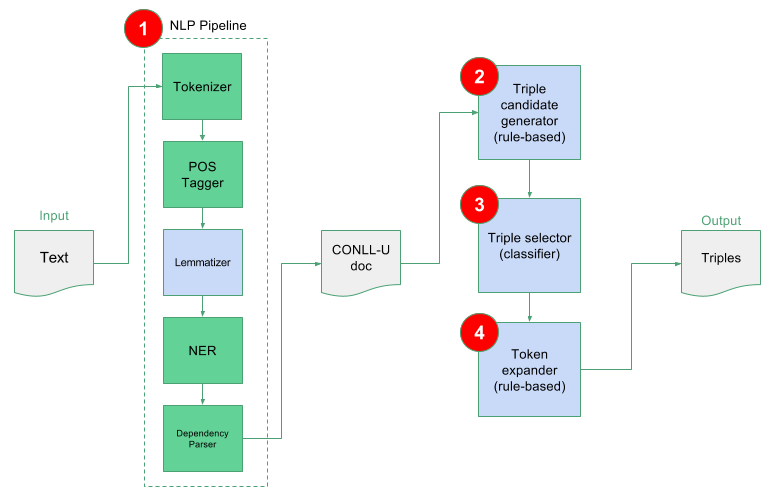
\includegraphics[width=0.50\textwidth]
		{../images/program_flowchart.png}
	\caption{\license.}
	\label{fig:testGambar}
\end{figure}


%-----------------------------------------------------------------------------%
\section{Membuat Tabel}
%-----------------------------------------------------------------------------%
Seperti pada gambar, tabel juga dapat diberi label dan caption. 
Caption pada tabel terletak pada bagian atas tabel. 
Contoh tabel sederhana dapat dilihat pada \tab~\ref{tab:tab1}.

\begin{table}
	\centering
	\caption{Contoh Tabel}
	\label{tab:tab1}
	\begin{tabular}{| l | c r |}
		\hline
		& kol 1 & kol 2 \\ 
		\hline
		baris 1 & 1 & 2 \\
		baris 2 & 3 & 4 \\
		baris 3 & 5 & 6 \\
		jumlah  & 9 & 12 \\
		\hline
	\end{tabular}
\end{table}

Ada jenis tabel lain yang dapat dibuat dengan \latex~berikut 
beberapa diantaranya. 
Contoh-contoh ini bersumber dari 
\url{http://en.wikibooks.org/wiki/LaTeX/Tables}

\begin{table}
	\centering
	\caption{An Example of Rows Spanning Multiple Columns}
	\label{row.spanning}
	\begin{tabular}{|l|l|*{6}{c|}}
  		\hline % create horizontal line
  		No & Name & \multicolumn{3}{|c|}{Week 1} & \multicolumn{3}{|c|}{Week 2} \\
  		\cline{3-8} % create line from 3rd column till 8th column
  		& & A & B & C & A & B & C\\
  		\hline
  		1 & Lala & 1 & 2 & 3 & 4 & 5 & 6\\
  		2 & Lili & 1 & 2 & 3 & 4 & 5 & 6\\
  		3 & Lulu & 1 & 2 & 3 & 4 & 5 & 6\\
  		\hline
	\end{tabular}
\end{table}

\begin{table}
	\centering
	\caption{An Example of Columns Spanning Multiple Rows}
	\label{column.spanning}
	\begin{tabular}{|l|c|l|}
		\hline
		Percobaan & Iterasi & Waktu \\
		\hline
		Pertama & 1 & 0.1 sec \\ \hline
		\multirow{2}{*}{Kedua} & 1 & 0.1 sec \\
 		& 3 & 0.15 sec \\ 
 		\hline
		\multirow{3}{*}{Ketiga} & 1 & 0.09 sec \\
 		& 2 & 0.16 sec \\
 		& 3 & 0.21 sec \\ 
 		\hline
	\end{tabular}
\end{table}

\begin{table}
	\centering
	\caption{An Example of Spanning in Both Directions Simultaneously}
	\label{mix.spanning}
	\begin{tabular}{cc|c|c|c|c|}
		\cline{3-6}
		& & \multicolumn{4}{|c|}{Title} \\ \cline{3-6}
		& & A & B & C & D \\ \hline
		\multicolumn{1}{|c|}{\multirow{2}{*}{Type}} &
		\multicolumn{1}{|c|}{X} & 1 & 2 & 3 & 4\\ \cline{2-6}
		\multicolumn{1}{|c|}{}                        &
		\multicolumn{1}{|c|}{Y} & 0.5 & 1.0 & 1.5 & 2.0\\ \cline{1-6}
		\multicolumn{1}{|c|}{\multirow{2}{*}{Resource}} &
		\multicolumn{1}{|c|}{I} & 10 & 20 & 30 & 40\\ \cline{2-6}
		\multicolumn{1}{|c|}{}                        &
		\multicolumn{1}{|c|}{J} & 5 & 10 & 15 & 20\\ \cline{1-6}
	\end{tabular}
\end{table}


%-----------------------------------------------------------------------------%
\chapter{\babTiga}
%-----------------------------------------------------------------------------%

Pada bab ini dijelaskan mengenai tahapan, rancangan \& implementasi sistem, pengumpulan \& pengolahan data dan teknik evaluasi yang digunakan pada penelitian ini.

%-----------------------------------------------------------------------------%
\section{Tahapan Penelitian}
%-----------------------------------------------------------------------------%

\lipsum[1-2]

%-----------------------------------------------------------------------------%
\section{Rancangan dan Implementasi Sistem}
%-----------------------------------------------------------------------------%

As shown in the flowchart Figure \ref{fig_program_flowchart}, our system is composed of four main components: \textbf{NLP pipeline}, \textbf{triple candidate generator}, \textbf{triple selector} and \textbf{token expander}. Each of them are explained further in following subsections.

\begin{figure}
\centering
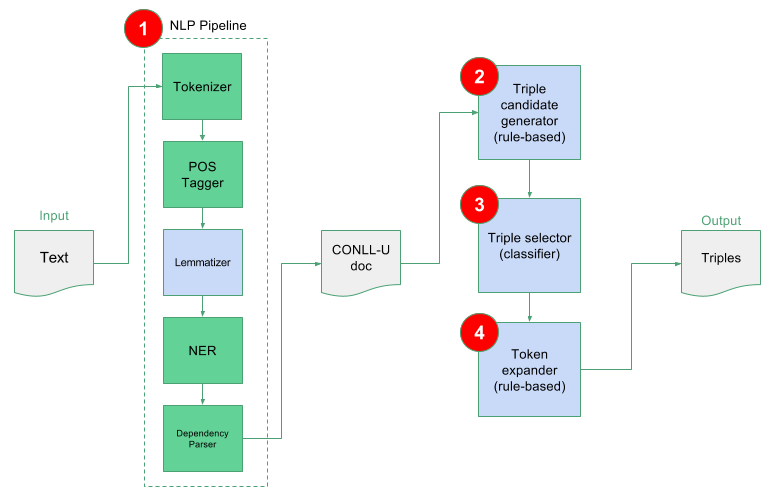
\includegraphics[width=\textwidth]{../images/program_flowchart.png}
\caption{Indonesian open domain information extraction flowchart}
\label{fig_program_flowchart}
\end{figure}

\subsection{NLP Pipeline}

The NLP pipeline is a series of NLP tasks that annotates one or more sentences and saves them in CONLL-U\footnote{CONLL-U format description \url{http://universaldependencies.org/format.html}} format, a token-based sentence annotation format containing lemma, POS tag, dependency relation and a slot for additional annotation. The pipeline assumes that each sentence in the input document is separated by new line so preprocessing may be required. The detail of each model the pipeline are described below:

\begin{enumerate}

\item Tokenizer \\
We use default tokenizer provided by Stanford Core NLP, \verb|PTBTokenizer| \citep{manningptbtokenizer}, which mimics Penn Treebank 3 tokenizer\footnote{Penn Treebank 3 \url{https://catalog.ldc.upenn.edu/LDC99T42}}. While this tokenizer provides many options to modify its behavior, we stick to default configuration that split sentence by whitelines to get the tokens.\\

\item Part of Speech Tagger \\
We trained default Stanford Core NLP \verb|MaxentTagger| \citep{toutanova2003feature} with Indonesian universal POS tag dataset which we convert from dependency parsing dataset\footnote{UD Indonesian dataset \url{https://github.com/UniversalDependencies/UD_Indonesian}}. This POS tagger uses Max Entropy (multi-class logistic regression) classifier which yields \textbf{93.68\%} token accuracy and \textbf{63.91\%} sentence accuracy when trained using 5,036 sentences and tested with 559 sentences from the dataset. \\

\item Lemmatizer \\
The lemmatizer used in this pipeline, \verb|IndonesianLemmaAnnotator|, is implemented based on an existing Indonesian rule-based Lemmatizer \citep{suhartono2014lemmatization} with some improvements:

\begin{itemize}
\item Ability to process a sentence instead of a token
\item Usage of in-memory database to speed up dictionary lookup
\item Reimplementation in Java language and integration with Stanford Core NLP annotator API to improve reusability
\end{itemize}

This lemmatizer yields \textbf{99\%} accuracy when tested using dataset of 5,638 token-lemma pairs\footnote{Indonesian Lemmatizer \url{https://github.com/davidchristiandy/lemmatizer}}. We use lemma as one of the features for NER classifier. \\

\item Named-Entity Recognizer (NER)

Stanford NLP \verb|CRFClassifier| \citep{finkel2005incorporating}, a linear chain Conditional Random Field (CRF) sequence models, is trained using a dataset containing 3,535 Indonesian sentences with 5 entity class: Person, Organization, Location, Quantity and Time. When tested using 426 sentences, this models achieves 0.86 precision, 0.85 recall and \textbf{0.86} F1-score. The dataset itself is a combination between dataset from Faculty of Computer Science, University of Indonesia and a public dataset\footnote{Indonesian NER \url{https://github.com/yusufsyaifudin/indonesia-ner}}. \\

\item Dependency Parser

We relied on Stanford NLP \verb|nndep.DependencyParser| \citep{chen2014fast}, to annotate dependency relation of each token in the sentence. We train this transition-based neural network model using a Indonesian universal dependencies dataset of 5,036 sentences and 3,093 Indonesian word embedding\footnote{Indonesian word embedding \url{https://github.com/yohanesgultom/id-openie/blob/master/data/parser-id.embed}} (vector representation of words). Tested with 559 sentences, this model scores \textbf{70\%} UAS (Unlabeled Attachment Score) and \textbf{46\%} LAS (Labeled Attachment Score).

\end{enumerate}

The output of the pipeline is a CONLL-U document containing annotated sentence such as Figure \ref{fig_conllu_example}. The document becomes an input for next model, the triple candidate generator which is described in Section \ref{Triple Candidates Generator}. Since the annotations that are directly used by following process are POS tag, named entity and dependency relation, we estimate that the accuracy of this NLP pipeline is \textbf{65.30\%} which comes from the average of POS tagger sentence accuracy, NER F1-score (in percent) and dependency parser LAS. Additionally, this pipeline is built by extending Stanford Core NLP classes and packaged as single Java program (JAR) to improve reusability.

\begin{figure}
\centering
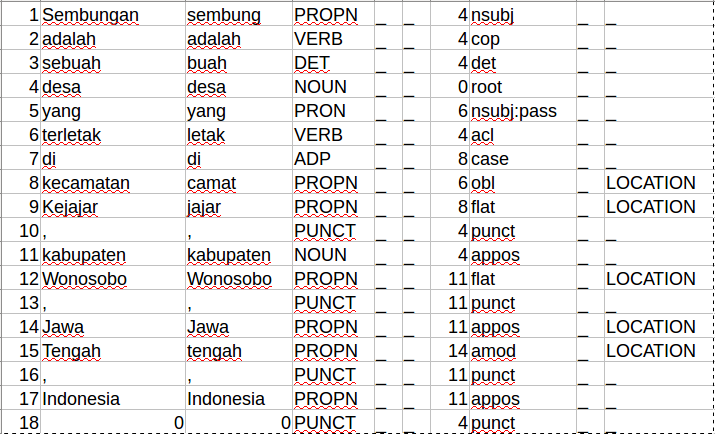
\includegraphics[scale=0.35]{../images/conllu_example.png}
\caption{Example of CONLL-U sentence annotation format}
\label{fig_conllu_example}
\end{figure}

\subsection{Triple Candidates Generator} \label{Triple Candidates Generator}

% Similar to TextRunner Self-Supervised Learner but doesn't automatically label triples

Triple candidates generator is used to extract relation triples candidates from CONLL-U document produced by NLP pipeline. It uses a set of rules listed in Table \ref{table_triple_candidate_generation_rules} to extract relations (predicates) and arguments (subjects and predicates) from the sentence. The results of triples extraction are not always the positive or valid relation triples so, unlike TextRunner \citep{banko2007open}, we cannot use them directly as training data for triple selector/classifier.

For example, applying the rules to an annotated sentence in Figure \ref{fig_conllu_example} will generate these 17 triples candidates where only five of them are valid triples (check-marked):

\begin{itemize}
\item (Sembungan, adalah, desa) \ding{51}
\item (Sembungan, adalah, terletak)
\item (Sembungan, adalah, kecamatan)
\item (Sembungan, adalah, kabupaten)
\item (Sembungan, adalah, Jawa)
\item (Sembungan, adalah, Tengah)
\item (Sembungan, adalah, Indonesia)
\item (Sembungan, terletak, kecamatan) \ding{51}
\item (Sembungan, terletak, kabupaten) \ding{51}
\item (Sembungan, terletak, Jawa) \ding{51}
\item (Sembungan, terletak, Tengah)
\item (Sembungan, terletak, Indonesia) \ding{51}
\item (desa, terletak, kecamatan)
\item (desa, terletak, kabupaten)
\item (desa, terletak, Jawa)
\item (desa, terletak, Tengah)
\item (desa, terletak, Indonesia)
\end{itemize}

In order to build a training data for the triple selector, we used triple candidates generator to generate 1,611 triple candidates from 42 sentences. As part of the label step, we manually label \textbf{132 positive} and \textbf{1,479 negative} triples which we use to train binary classifier as triple selector in the learn step.

During the extraction step, triple candidates generator is used in the system to extract unlabeled candidates from CONLL-U document. These unlabeled triples will be labeled by trained triple selector as described in  (referring to flowchart in Figure \ref{fig_program_flowchart}).

% Triple candidate generation rules
\begin{table}[!t]
\renewcommand{\arraystretch}{1.5}
\caption{Triple candidate generation rules}
\label{table_triple_candidate_generation_rules}
\centering
\begin{tabular}{l p{6cm}}
\hline
\textbf{Type} & \textbf{Condition} \\
\hline
Subject & Token's POS tag is either PROPN, NOUN, PRON or VERB \\
\space & Token is not "yang" nor "adalah" \\
\space & Token's dependency is neither "compound" nor "name" \\
\space & Token's dependency is either "compound" or "name" but separated by more than 2 tokens from its head \\
\hline
Predicate & Token's position is after Subject \\
\space & Token's POS tag is either VERB or AUX \\
\hline
Object & Token's position is after Subject and Predicate \\
\space & Token's POS tag is either PROPN, NOUN, PRON or VERB \\
\space & Token is not "yang" nor "adalah" \\
\space & Token's dependency is neither "compound" nor "name" \\
\space & Token's dependency is either "compound" or "name" but separated by more than 2 tokens from its head \\
\end{tabular}
\end{table}


\subsection{Triple Selector}  \label{Triple Selector}

Triple selector is a machine learning classifier trained using manually labeled dataset of valid and invalid relation triples. For example, given the input of 17 candidates in Section \ref{Triple Candidates Generator}, the selector will label the five check-marked triples as true and label the rest as false.

We use Random Forest \citep{breiman2001random}, an ensemble methods that aggregate classification results from multiple decision trees, as the model for the classifier. We use the Scikit-Learn\footnote{scikit-learn: machine learning in Python \url{http://scikit-learn.org}} implementation of Random Forest with following configuration:

\begin{itemize}
\item Decision tree criterion: Gini Impurity
\item Minimum number of samples to split tree node: 5 samples
\item Maximum features used in each tree: 4 (square root of the number of features)
\item Maximum trees depth: 8
\item Number of trees: 20
\item Class weight: balanced (prediction probability is multiplied by the ratio of training samples)
\end{itemize}

We discover the configuration by using Grid Search \citep{wasserman2015grid}, an exhaustive search algorithm to find optimal hyper-parameters, to find the best F1 score for Random Forest classifier using dataset described in Section \ref{Triple Candidates Generator}. 

We extract 17 features described in Table \ref{table_models_features} from each triple candidates. These features are based on POS tag, named-entity and dependency relation, instead of shallow syntactic features used by TextRunner or ReVerb \citep{banko2007open} \citep{etzioni2011open}. Every nominal features are also encoded and normalized along with the whole dataset by removing the mean and scaling to unit variance in order to improve the precision and recall of the classifier.

\begin{table}[!t]
\renewcommand{\arraystretch}{1.5}
\caption{Triple selector features}
\label{table_models_features}
\centering
\begin{tabular}{r l}
\hline
\textbf{\#} & \textbf{Triple Features} \\
\hline
1 & Subject token's POS tag \\
2 & Subject token's dependency relation \\
3 & Subject token's head POS tag \\
4 & Subject token's named entity \\
5 & Subject token's distance from predicate \\
6 & Subject token's dependency with predicate \\
7 & Predicate token's POS tag \\
8 & Predicate token's dependency relation \\
9 & Predicate token's head POS tag \\
10 & Predicate token's dependents count \\
11 & Object token's POS tag \\
12 & Object token's dependency relation \\
13 & Object token's head POS tag \\
14 & Object token's named entity \\
15 & Object token's dependents count \\
16 & Object token's distance from predicate \\
17 & Object token's dependency with predicate \\
\end{tabular}
\end{table}

During the train step, we use the dataset to train triple selector and save the best model as binary file. This model is included in the system to be use during the extraction step.

\subsection{Token Expander}

Instead of using lightweight noun phrase chunker \citep{banko2007open}, our system uses rule-based token expander to extract relation or argument clauses. While having different objective and approach, this token expander works similarly to Clause Selector in Stanford Open IE \citep{angeli2015leveraging} where the algorithm starts from a token then decides whether to expand to its dependents. Instead of using machine learning model like Clause Selector, it uses simple heuristics based on syntactical features (POS tag, dependency relation and named-entity) described in Table \ref{table_token_expansion_rules_s_o} and Table \ref{table_token_expansion_rules_p} to determine whether to: (1) expand a token to its dependent, (2) ignore the dependent or (3) remove the token itself. For example, token expander will expand check-marked triples in Section \ref{Triple Candidates Generator} into:

\begin{itemize}
\item (Sembungan, adalah, desa)
\item (Sembungan, terletak di, kecamatan Kejajar)
\item (Sembungan, terletak di, kabupaten Wonosobo)
\item (Sembungan, terletak di, Jawa Tengah)
\item (Sembungan, terletak di, Indonesia)
\end{itemize}

% Token expansion rules for Subject or Object token
\begin{table}[!t]
\renewcommand{\arraystretch}{1.5}
\caption{Token expansion rules for Subject or Object token}
\label{table_token_expansion_rules_s_o}
\centering
\begin{tabular}{r p{6cm} l}
\hline
\textbf{\#} & \textbf{Condition for Subject or Object Token} & \textbf{Action} \\
\hline
1 & If dependent's relation to the token  is either “compound”, “name”  or “amod” & Expand \\
2 & If dependent has same named entity as the token & Expand \\
3 & If dependent and the token are wrapped by quotes or double quotes  & Expand \\
4 & If the head is a sentence root & Ignore \\
5 & If dependent's POS tag is CONJ or its form is either “,” (comma) or “/” (slash) & Ignore \\
6 & If dependent's POS tag is either “VERB” or “ADP” & Ignore \\
7 & If dependent has at least one dependent with “ADP” POS tag & Ignore \\
8 & If the first or last token in expansion result has “CONJ” or “ADP” POS tag & Remove \\
9 & If the first or last index of expansion result is an incomplete parentheses symbol & Remove \\
10 & If the last index of expansion result is “yang” & Remove \\
11 & Else & Ignore \\
\hline
\end{tabular}
\end{table}

\begin{table}[!t]
\renewcommand{\arraystretch}{1.5}
\caption{Token expansion rules for Predicate token}
\label{table_token_expansion_rules_p}
\centering
\begin{tabular}{r p{6cm} l}
\hline
\textbf{\#} & \textbf{Condition for Predicate Token} & \textbf{Action} \\
\hline
1 & If dependent is “tidak” & Expand \\
2 & Else & Ignore \\
\hline
\end{tabular}
\end{table}

During the label step, token expander is used to make manual annotation process easier. We label a triple candidate as valid only if it makes sense after being expanded to clause. For example, \textit{(Sembungan, terletak, kecamatan)} doesn't seem to make sense before expanded to \textit{(Sembungan, terletak di, kecamatan Kejajar)}.
%-----------------------------------------------------------------------------%
\chapter{\babEmpat}
%-----------------------------------------------------------------------------%
\todo{tambahkan kata-kata pengantar bab 1 disini}

%-----------------------------------------------------------------------------%
\section{thesis.tex}
%-----------------------------------------------------------------------------%
Berkas ini berisi seluruh berkas Latex yang dibaca, jadi bisa dikatakan sebagai 
berkas utama. Dari berkas ini kita dapat mengatur bab apa saja yang ingin 
kita tampilkan dalam dokumen.


%-----------------------------------------------------------------------------%
\section{laporan\_setting.tex}
%-----------------------------------------------------------------------------%
Berkas ini berguna untuk mempermudah pembuatan beberapa template standar. 
Anda diminta untuk menuliskan judul laporan, nama, npm, dan hal-hal lain yang 
dibutuhkan untuk pembuatan template. 


%-----------------------------------------------------------------------------%
\section{istilah.tex}
%-----------------------------------------------------------------------------%
Berkas istilah digunakan untuk mencatat istilah-istilah yang digunakan. 
Fungsinya hanya untuk memudahkan penulisan.
Pada beberapa kasus, ada kata-kata yang harus selalu muncul dengan tercetak 
miring atau tercetak tebal. 
Dengan menjadikan kata-kata tersebut sebagai sebuah perintah \latex~tentu akan 
mempercepat dan mempermudah pengerjaan laporan. 


%-----------------------------------------------------------------------------%
\section{hype.indonesia.tex}
%-----------------------------------------------------------------------------%
Berkas ini berisi cara pemenggalan beberapa kata dalam bahasa Indonesia. 
\latex~memiliki algoritma untuk memenggal kata-kata sendiri, namun untuk 
beberapa kasus algoritma ini memenggal dengan cara yang salah. 
Untuk memperbaiki pemenggalan yang salah inilah cara pemenggalan yang benar 
ditulis dalam berkas hype.indonesia.tex.


%-----------------------------------------------------------------------------%
\section{pustaka.tex}
%-----------------------------------------------------------------------------%
Berkas pustaka.tex berisi seluruh daftar referensi yang digunakan dalam 
laporan. 
Anda bisa membuat model daftar referensi lain dengan menggunakan bibtex.
Untuk mempelajari bibtex lebih lanjut, silahkan buka 
\url{http://www.bibtex.org/Format}. 
Untuk merujuk pada salah satu referensi yang ada, gunakan perintah \bslash 
cite, e.g. \bslash cite\{latex.intro\} yang akan akan memunculkan 
\cite{latex.intro}


%-----------------------------------------------------------------------------%
\section{bab[1 - 6].tex}
%-----------------------------------------------------------------------------%
Berkas ini berisi isi laporan yang Anda tulis. 
Setiap nama berkas e.g. bab1.tex merepresentasikan bab dimana tulisan tersebut 
akan muncul. 
Sebagai contoh, kode dimana tulisan ini dibaut berada dalam berkas dengan nama 
bab4.tex. 
Ada enam buah berkas yang telah disiapkan untuk mengakomodir enam bab dari 
laporan Anda, diluar bab kesimpulan dan saran. 
Jika Anda tidak membutuhkan sebanyak itu, silahkan hapus kode dalam berkas 
thesis.tex yang memasukan berkas \latex~yang tidak dibutuhkan;  contohnya 
perintah \bslash include\{bab6.tex\} merupakan kode untuk memasukan berkas 
bab6.tex kedalam laporan.

%-----------------------------------------------------------------------------%
\section{Penulisan \textit{code} atau \textit{pseudocode} program}
%-----------------------------------------------------------------------------%

\subsection{\textit{Inline}}

Dengan perintah \verb|\verb|: \verb|System.out.println("Hello, World");| \\
Dengan perintah \textit{custom} \verb|\code|: \code{	System.out.println("Hello, World"); }

\subsection{\textit{Multiline}}

Dengan perintah \verb|verbatim|: 

\begin{verbatim}	
public class HelloWorld {
    public static void main(String[] args) {
        // Prints "Hello, World" to the terminal window.
        System.out.println("Hello, World");
    }
}
\end{verbatim}

Dengan perintah \verb|lstlisting|:

\begin{lstlisting}[language=Java]
public class HelloWorld {
 public static void main(String[] args) {
     // Prints "Hello, World" to the terminal window.
     System.out.println("Hello, World");
 }
}
\end{lstlisting}

Konfigurasi tampilan bisa dilakukan di \verb|uithesis.sty| dengan referensi dokumentasi di \url{https://en.wikibooks.org/wiki/LaTeX/Source_Code_Listings}
%-----------------------------------------------------------------------------%
\chapter{\babLima}
%-----------------------------------------------------------------------------%
\todo{Tambahkan kata-kata pengantar bab 5 disini.}


%-----------------------------------------------------------------------------%
\section{Mengubah Tampilan Teks}
%-----------------------------------------------------------------------------%
Beberapa perintah yang dapat digunakan untuk mengubah tampilan adalah: 
\begin{itemize}
	\item \bslash f \\
		Merupakan alias untuk perintah \bslash textit, contoh 
		\f{contoh hasil tulisan}.
	\item \bslash bi \\
		\bi{Contoh hasil tulisan}.
	\item \bslash bo \\
		\bo{Contoh hasil tulisan}.
	\item \bslash m \\
		\m{Contoh hasil tulisan}.
	\item \bslash mc \\
		\mc{Contoh hasil tulisan}.
	\item \bslash code \\ 
		\code{Contoh hasil tulisan}.
\end{itemize}


%-----------------------------------------------------------------------------%
\section{Memberikan Catatan}
%-----------------------------------------------------------------------------%
Ada dua perintah untuk memberikan catatan penulisan dalam dokumen yang Anda 
kerjakan, yaitu: 
\begin{itemize}
	\item \bslash todo \\
		Contoh: \\ \todo{Contoh bentuk todo.}
	\item \bslash todoCite \\ 
		Contoh: \todoCite
\end{itemize}


%-----------------------------------------------------------------------------%
\section{Menambah Isi Daftar Isi}
%-----------------------------------------------------------------------------%
Terkadang ada kebutuhan untuk memasukan kata-kata tertentu kedalam Daftar Isi. 
Perintah \bslash addChapter dapat digunakan untuk judul bab dalam Daftar isi. 
Contohnya dapat dilihat pada berkas thesis.tex.


%-----------------------------------------------------------------------------%
\section{Memasukan PDF}
%-----------------------------------------------------------------------------%
Untuk memasukan PDF dapat menggunakan perintah \bslash inpdf yang menerima satu 
buah argumen. Argumen ini berisi nama berkas yang akan digabungkan dalam 
laporan. PDF yang dimasukan degnan cara ini akan memiliki header dan footer 
seperti pada halaman lainnya. 

\inpdf{include}

Cara lain untuk memasukan PDF adalah dengan menggunakan perintah \bslash putpdf 
dengan satu argumen yang berisi nama berkas pdf. Berbeda dengan perintah 
sebelumnya, PDF yang dimasukan dengan cara ini tidak akan memiliki footer atau 
header seperti pada halaman lainnya. 

\putpdf{include}


%-----------------------------------------------------------------------------%
\section{Membuat Perintah Baru}
%-----------------------------------------------------------------------------%
Ada dua perintah yang dapat digunakan untuk membuat perintah baru, yaitu: 
\begin{itemize}
	\item \bslash Var \\
		Digunakan untuk membuat perintah baru, namun setiap kata yang diberikan
		akan diproses dahulu menjadi huruf kapital. 
		Contoh jika perintahnya adalah \bslash Var\{adalah\} makan ketika 
		perintah \bslash Var dipanggil, yang akan muncul adalah ADALAH. 
	\item \bslash var \\
		Digunakan untuk membuat perintah atau baru. 
\end{itemize}



%
% Daftar Pustaka
%\include{pustaka}

% Alternatif manajemen daftar pustaka dengan \bibliography
\bibliographystyle{apalike}
\bibliography{../pustaka}

%
% Lampiran 
%
\begin{appendix}
	%
% @author  Andreas Febrian
% @version 1.00 
% 
% Hanya sebuah pembatas bertuliskan LAMPIRAN ditengah halaman. 
% 

\begin{titlepage}
	\centering 
	\vspace*{6cm}
	\noindent \Huge{LAMPIRAN}
	\addChapter{LAMPIRAN}
\end{titlepage}
	\setcounter{page}{2}
	%-----------------------------------------------------------------------------%
\addChapter{Lampiran 1: Kode Sumber Program Utama}
%-----------------------------------------------------------------------------%

\chapter*{Lampiran 1: Kode Sumber Program Utama}

Kode sumber program utama (\textit{main program}) \verb|extract_triples.py|

\begin{lstlisting}[language=Python]
import os
import csv
import argparse
import subprocess
import numpy as np
import json
from sys import platform
from sklearn.externals import joblib
from sklearn.preprocessing import StandardScaler
from tripletools import (
    vectorize,
    parse_connlu_file,
    extract_triples_by_combinations,
    get_best_features
)
from pprint import pprint

# choose script based on OS (windows or *nix)
DEPPARSE_SCRIPT = 'bin' + os.sep + 'id-openie'
if platform == 'win32':
    DEPPARSE_SCRIPT += '.bat'


def write_json(triples, y, out):
    count = 0
    grouped = {}
    for i in range(y.shape[0]):
        if y[i] == 1:
            triple = triples[i]
            if triple[1] not in grouped:
                grouped[triple[1]] = {}
            if triple[2] not in grouped[triple[1]]:
                grouped[triple[1]][triple[2]] = {}
            if triple[3] not in grouped[triple[1]][triple[2]]:
                grouped[triple[1]][triple[2]][triple[3]] = {}
            count += 1
    out.write(json.dumps(grouped) + '\n')
    return count


def write_tsv(triples, y, out):
    writer = csv.writer(out, delimiter='\t', quoting=csv.QUOTE_NONE, quotechar='')
    count = 0
    for i in range(y.shape[0]):
        if y[i] == 1:
            writer.writerow(triples[i])
            count += 1
    return count


def extract(conllu_file, classifier, out, format='tsv', scaler=None):
    X = []
    triples = []
    for index, s, s_header in parse_connlu_file(conllu_file):
        for first, second, third, subj, pred, obj in extract_triples_by_combinations(s, s_header):
            X.append(vectorize(first, second, third))
            triples.append((first['sentence_id'], subj, pred, obj))
    X = np.array(X, dtype='float32')
    # apply best features selection
    X = X[:, get_best_features()]
    # scale if scaler is available
    if scaler:
        X = scaler.transform(X)
    y = classifier.predict(X)
    # write output
    if format == 'tsv':
        return write_tsv(triples, y, out)
    else:  # format == 'json'
        return write_json(triples, y, out)


if __name__ == '__main__':

    if os.path.isfile(DEPPARSE_SCRIPT):
        parser = argparse.ArgumentParser(description='Extract triples from Indonesian text')
        parser.add_argument('input_file', help='Input file containing 1 (one) Indonesian sentence per line')
        parser.add_argument('-m', '--model_file', help='Triples classifier model file', default='triples-classifier-model.pkl')
        parser.add_argument('-s', '--scaler_file', help='Triples classifier scaler file', default='triples-classifier-scaler.pkl')
        parser.add_argument('-o', '--output_file', help='Output file containing triples')
        parser.add_argument('-f', '--output_format', help='Output file format', choices=['json', 'tsv'], default='json')
        args = parser.parse_args()
        args.output_file = args.output_file if args.output_file else 'triples.' + args.output_format

        # dependency parsing
        print('Parsing dependency tree..')
        depparse_output = os.path.basename(args.input_file) + '.conllu'
        subprocess.call([DEPPARSE_SCRIPT, '-f', args.input_file])

        # extract triples
        classifier = joblib.load(args.model_file)
        scaler = joblib.load(args.scaler_file)
        with open(args.output_file, 'wb') as out:
            count = extract(depparse_output, classifier, out, args.output_format, scaler=scaler)

        print('{} triple(s) extracted'.format(count))
        print('Triples saved in ' + args.output_file)
    else:
        print('File not found: ' + DEPPARSE_SCRIPT)
\end{lstlisting}

%-----------------------------------------------------------------------------%
\addChapter{Lampiran 2: Kode Sumber \textit{NLP Pipeline}}
%-----------------------------------------------------------------------------%

\chapter*{Lampiran 2: Kode Sumber \textit{NLP Pipeline}}

Kode sumber utama \textit{NLP pipeline}: \verb|DepdendencyParser.java|

\begin{lstlisting}[language=Java]
package id.nlp.depparser;

import edu.stanford.nlp.ling.CoreAnnotations;
import edu.stanford.nlp.pipeline.*;
import edu.stanford.nlp.semgraph.SemanticGraph;
import edu.stanford.nlp.semgraph.SemanticGraphCoreAnnotations;
import edu.stanford.nlp.trees.ud.CoNLLUDocumentWriter;
import edu.stanford.nlp.trees.ud.ExtendedCoNLLUDocumentWriter;
import edu.stanford.nlp.util.CoreMap;
import edu.stanford.nlp.util.PropertiesUtils;
import net.sourceforge.argparse4j.ArgumentParsers;
import net.sourceforge.argparse4j.inf.ArgumentParser;
import net.sourceforge.argparse4j.inf.ArgumentParserException;
import net.sourceforge.argparse4j.inf.Namespace;

import java.io.File;
import java.io.IOException;
import java.sql.SQLException;
import java.util.ArrayList;
import java.util.List;
import java.util.Properties;

import static edu.stanford.nlp.pipeline.Annotator.*;

public class DependencyParser {

    static final String TAGGER_MODEL = "tagger-id.universal.model";
    static final String NER_MODEL = "ner-id.model.ser.gz";
    static final String PARSER_MODEL = "parser-id.conllu.model.gz";
    static final int NUM_THREADS = 1;
    static final String OUTPUT_FORMAT = "conllu";

    AnnotatorPool annotatorPool;
    Properties props;
    StanfordCoreNLP pipeline;

    public DependencyParser() throws SQLException, IOException, ClassNotFoundException {
        this(TAGGER_MODEL, NER_MODEL, PARSER_MODEL, NUM_THREADS);
    }

    public DependencyParser(
            String taggerModel,
            String nerModel,
            String parserModel,
            int numThreads
    ) throws SQLException, IOException, ClassNotFoundException {

        // Create the Stanford CoreNLP pipeline
        this.props = PropertiesUtils.asProperties(
                "annotators", "tokenize,ssplit,pos,lemma,ner,depparse",
                "ssplit.eolonly", "true",
                "ner.model", nerModel,
                "ner.useSUTime", "false",
                "pos.model", taggerModel,
                "depparse.model", parserModel,
                "splitter.nomodel", "true",
                "ignore_affinity", "true",
                "outputFormat", OUTPUT_FORMAT,
                "threads", String.valueOf(numThreads)
        );

        // Create annotator pools
        this.annotatorPool = new AnnotatorPool();
        AnnotatorImplementations annotatorImplementations = new IndonesianAnnotatorImplementations();
        annotatorPool.register(STANFORD_TOKENIZE, AnnotatorFactories.tokenize(props, annotatorImplementations));
        annotatorPool.register(STANFORD_SSPLIT, AnnotatorFactories.sentenceSplit(props, annotatorImplementations));
        annotatorPool.register(STANFORD_POS, AnnotatorFactories.posTag(props, annotatorImplementations));
        annotatorPool.register(STANFORD_LEMMA, AnnotatorFactories.lemma(props, annotatorImplementations));
        annotatorPool.register(STANFORD_NER, AnnotatorFactories.nerTag(props, annotatorImplementations));
        annotatorPool.register(STANFORD_DEPENDENCIES, AnnotatorFactories.dependencies(props, annotatorImplementations));

        // Create pipeline
        this.pipeline = new IndonesianStanfordCoreNLP(this.props, annotatorPool);
    }

    /**
     * Parse text
     * @param text
     * @return
     */
    public String parse(String text) {
        StringBuilder result = new StringBuilder();
        Annotation doc = pipeline.process(text);
        List<CoreMap> sentences = doc.get(CoreAnnotations.SentencesAnnotation.class);
        CoNLLUDocumentWriter conllUWriter = new ExtendedCoNLLUDocumentWriter();
        for (CoreMap sentence : sentences) {
            SemanticGraph sg = sentence.get(SemanticGraphCoreAnnotations.BasicDependenciesAnnotation.class);
            if (sg != null) {
                result.append(conllUWriter.printSemanticGraph(sg)).append("\n");
            }
        }
        return result.toString();
    }

    /**
     * Parse input file(s)
     * @param inputFiles
     * @param outputDir
     * @throws IOException
     */
    public void parse(List<File> inputFiles, String outputDir) throws IOException, SQLException, ClassNotFoundException {
        // override existing pipeline
        if (!props.containsKey("outputDirectory")) {
            props.setProperty("outputDirectory", outputDir);
            this.pipeline = new IndonesianStanfordCoreNLP(this.props, this.annotatorPool);
        }
        pipeline.processFiles(inputFiles);
    }

    public static void main(String args[]) {

        // parse arguments
        ArgumentParser parser = ArgumentParsers.newArgumentParser("DependencyParser").defaultHelp(true).description("Generate CONLL-U dependency tree from Indonesian text");
        parser.addArgument("-t", "--text").help("Text input to parse");
        parser.addArgument("-f", "--file").nargs("*").help("File input to parse");
        parser.addArgument("-o", "--outputDir").setDefault(".").help("Output directory");

        Namespace ns = null;
        try {
            ns = parser.parseArgs(args);
        } catch (ArgumentParserException e) {
            parser.handleError(e);
            System.exit(1);
        }

        String text = ns.getString("text");
        List<String> files = ns.<String> getList("file");
        String outputDir = ns.getString("outputDir");
        try {
            if (text != null) {
                text = text.trim();
                if (!text.endsWith(".")) {
                  text += ".";
                }
                System.out.println(new DependencyParser().parse(text));
            } else if (files != null) {
                List<File> fileList = new ArrayList<>();
                List<String> outputFiles = new ArrayList<>();
                String sep = System.getProperty("file.separator");
                for (String file:files) {
                    File fileObj = new File(file);
                    fileList.add(fileObj);
                    outputFiles.add(outputDir + sep + fileObj.getName() + "." + OUTPUT_FORMAT);
                }
                new DependencyParser().parse(fileList, outputDir);
                System.out.println("File(s) created:");
                for (String outputFile:outputFiles) {
                    System.out.println(outputFile);
                }
            } else {
                System.err.println("No input provided");
            }
        } catch (Exception e) {
            e.printStackTrace();
        }
    }
}

\end{lstlisting}


%-----------------------------------------------------------------------------%
\addChapter{Lampiran 3: Kode Sumber Pustaka Utama}
%-----------------------------------------------------------------------------%

\chapter*{Lampiran 3: Kode Sumber Pustaka Utama}

Kode sumber pustaka utama (\textit{main library}) yang berisi kode sumber untuk \textit{Triple Candidates Generator}, \textit{Token Expander} dan \textit{Triple Selector} \verb|tripletools.py|

\begin{lstlisting}[language=Python]
import itertools
import csv
import argparse


BEST_FEATURES = [0, 1, 2, 3, 5, 6, 10, 11, 12, 14, 17, 18, 19, 20, 21, 22, 23]  # F1 0.586
# BEST_FEATURES = [0, 1, 2, 3, 5, 6, 10, 11, 12, 17, 18, 19, 20, 21, 22, 23]   # F1 0.579
# BEST_FEATURES = [0, 1, 2, 3, 4, 5, 6, 7, 8, 9, 10, 11, 12, 13, 14, 15, 16, 17, 18, 19, 20, 21, 22, 23, 24, 25, 26]  # F1 0.547


# constants
conllu = ['ID', 'FORM', 'LEMMA', 'UPOSTAG', 'XPOSTAG', 'FEATS', 'HEAD', 'DEPREL', 'DEPS', 'MISC']
postag = ['', 'ADJ', 'ADP', 'ADV', 'AUX', 'CCONJ', 'DET', 'INTJ', 'NOUN', 'NUM', 'PART', 'PRON', 'PROPN', 'PUNCT', 'SCONJ', 'SYM', 'VERB', 'X', 'CONJ']
deprel = ['', 'acl', 'advcl', 'advmod', 'amod', 'appos', 'aux', 'case', 'cc', 'ccomp', 'clf', 'compound', 'conj', 'cop', 'csubj', 'dep', 'det', 'discourse', 'dislocated', 'expl', 'fixed', 'flat', 'goeswith', 'iobj', 'list', 'mark', 'nmod', 'nsubj', 'nummod', 'obj', 'obl', 'orphan', 'parataxis', 'punct', 'reparandum', 'root', 'vocative', 'xcomp', 'nsubjpass', 'name', 'dobj', 'neg', 'mwe', 'csubjpass']
entity = ['', 'PERSON', 'LOCATION', 'ORGANIZATION', 'TIME', 'QUANTITY', 'OTHER']

# extraction RULES
subject_object_candidates_pos = ['PROPN', 'NOUN', 'PRON', 'VERB']
predicate_candidates_pos = ['VERB', 'AUX']
non_subject_object_candidates_form = ['yang', 'adalah']
non_predicate_candidates_form = ['yang']
num_siblings = 1  # bigram


def extract_triples_by_root_children(conllu_s, header):
    """
    Extract features (triples) for clustering from sentence (conllu_s)
    by combining sentence root/header with 2 of its children
    """
    # find all direct branches of header
    direct_branches = []
    for id, row in conllu_s.iteritems():
        # children (direct branches of header)
        if (
            row['head'] == header['id'] and
            row['upostag'] in subject_object_candidates_pos and
            row['form'] not in non_subject_object_candidates_form
        ):
            direct_branches.append(id)

    # yield triples combinations
    if len(direct_branches) > 1:
        for combi in itertools.combinations(direct_branches, 2):
            first = None
            third = None
            if combi[0] < header['id'] and header['id'] < combi[1]:
                first = conllu_s[combi[0]]
                third = conllu_s[combi[1]]
            elif combi[1] < header['id'] and header['id'] < combi[0]:
                first = conllu_s[combi[1]]
                third = conllu_s[combi[0]]

            if first and third:
                second = conllu_s[header['id']]
                yield (first, second, third)


def extract_triples_by_combinations(conllu_s, header):
    """
    Extract features (triples) for clustering from sentence (conllu_s)
    by enumerating all possible triple combination of word
    """
    num_tokens = len(conllu_s)
    # sentence start from 1
    for i in range(1, num_tokens - 2):
        first = conllu_s[i]
        # RULES for Subject
        if (
            first['upostag'] in subject_object_candidates_pos and
            first['form'] not in non_subject_object_candidates_form and
            (first['deprel'] not in ['compound', 'name'] or first['head_distance'] > 2)
        ):
            for j in range(i + 1, num_tokens - 1):
                second = conllu_s[j]
                # RULES for Predicate
                if (
                    second['upostag'] in predicate_candidates_pos
                ):
                    for k in range(j + 1, num_tokens):
                        third = conllu_s[k]
                        # RULES for Object
                        if (
                            third['upostag'] in subject_object_candidates_pos and
                            third['form'] not in non_subject_object_candidates_form and
                            (third['deprel'] not in ['compound', 'name'] or third['head_distance'] > 2) and
                            (third['upostag'] not in predicate_candidates_pos or first['upostag'] not in predicate_candidates_pos)
                        ):
                            s = first['flatten_s']
                            p = second['flatten_p']
                            if third['nearest_adp_id']:
                                p += ' ' + conllu_s[third['nearest_adp_id']]['form']
                            o = third['flatten_o']
                            yield (first, second, third, s, p, o)


def extract_triples_by_children_combination(conllu_s, header):
    """
    Extract features (triples) for clustering from sentence (conllu_s)
    by combining sentence predicate nodes with 2 of their children
    """
    for k, v in conllu_s.items():
        # RULES for Subject, Predicate and Object
        if (
            v['upostag'] in predicate_candidates_pos and
            v['form'] not in non_predicate_candidates_form
        ):
            for first, second, third in extract_triples_by_root_children(conllu_s, v):
                yield (first, second, third)


def trace_children_pos(child_pos_list, parent_pos, node, s):
    """
    Find parent that has parent_pos pos tag and has one child of child_pos
    """
    parent_pos_list = [parent_pos] if parent_pos not in ['NOUN', 'PROPN'] else ['NOUN', 'PROPN']
    if node['deprel'] == 'root' or node['upostag'] not in parent_pos_list:
        return None
    else:
        # find child with upostag == child_pos
        for child_id in node['children']:
            if s[child_id]['upostag'] in child_pos_list:
                return s[child_id]

        # if not found try to search on node's parent
        return trace_children_pos(child_pos_list, parent_pos, s[node['head']], s)


def remove_token_if_first(field, values, tokens):
    while (tokens and tokens[0][1][field] in values):
        tokens.pop(0)


def remove_token_if_last(field, values, tokens):
    while (tokens and tokens[-1][1][field] in values):
        tokens.pop(-1)


def remove_token_if_first_or_last(field, values, tokens):
    remove_token_if_first(field, values, tokens)
    remove_token_if_last(field, values, tokens)


def expand_node(node, s):
    """
    Expand node to its children as dict
    """
    expanded = {node['id']: node}
    has_quote = False
    # EXPAND RULES

    for k in node['children']:
        v = s[k]
        if v['deprel'] in ['compound', 'name', 'amod']:
            expanded.update(expand_node(v, s))
        elif v['entity'] and v['entity'] == node['entity'] and abs(v['id'] - node['id']) == 1:
            expanded.update(expand_node(v, s))
        elif has_quote:
            expanded.update(expand_node(v, s))
        elif node['deprel'] == 'root':     # [Sembungan adalah sebuah] (desa) [.]
            continue
        else:
            if v['form'] in ['\'', '"']:  # (" Lelaki dan Telaga ")
                has_quote = True
            if (v['upostag'] in ['CONJ'] or v['form'] in [',', '/']):  # (kecamatan) Kejajar [, kabupaten Wonosobo]
                break
            if v['upostag'] in ['VERB', 'ADP']:  # (helm) Brodie [yang dipakai]
                continue
            if v['children'] and 'ADP' in [s[i]['upostag'] for i in v['children']]:  # (Stahlhelm) Jerman [dengan perbaikan desain], [Beberapa bulan sebelum] (Rose)
                continue
            expanded.update(expand_node(v, s))

    return expanded


def flatten_node(node, s, expand_as='o', mark_head=False):
    """
    Expand node and its branches to clause string
    """
    if expand_as.lower() in ['s', 'o']:
        expanded = expand_node(node, s)
        sorted_nodes = sorted(expanded.items())

        # EXPAND RULES
        remove_token_if_first_or_last('upostag', ['CONJ', 'ADP'], sorted_nodes)
        remove_token_if_first('form', [')'], sorted_nodes)
        remove_token_if_last('form', ['(', 'yang'], sorted_nodes)

        text = ' '.join([v['form'] if not mark_head or k != node['id'] else '({})'.format(v['form']) for k, v in sorted_nodes])
        ids = [k for k, v in sorted_nodes]
    elif expand_as.lower() in ['p']:
        text = node['form'] if not mark_head else '({})'.format(node['form'])
        ids = [node['id']]

        # EXPAND RULES
        negation_node = [s[c_id] for c_id in node['children'] if s[c_id]['form'].lower() == 'tidak']
        if negation_node:
            text = negation_node[0]['form'] + ' ' + text
            ids = [negation_node[0]['id']] + ids

    return text, ids


def flatten_conllu_sentence(conllu_s):
    return ' '.join([token['form'] for token in conllu_s.values()])


def set_extra_properties(s, children, mark_head=False):
    """
    Retrieve head's pos tag
    Flatten subject/object candidates
    """
    for k, v in s.iteritems():
        # get head pos tag
        s[k]['head_upostag'] = s[v['head']]['upostag'] if v['head'] > 0 else ''
        # get siblings pos tags
        before = v['id'] - num_siblings
        s[k]['before_upostag'] = [s[i]['upostag'] if i > 0 else '' for i in range(before, v['id'])]
        after = v['id'] + num_siblings + 1
        s[k]['before_upostag'] = [s[i]['upostag'] if i < len(s) else '' for i in range(after - num_siblings, after)]
        # get children id
        if k in children:
            sorted_children = sorted(children[k])
            s[k]['children'] = sorted_children

    # loop once more to flatten as children is required
    for k, v in s.iteritems():
        if v['upostag'] in subject_object_candidates_pos:
            s[k]['flatten_s'], s[k]['flatten_s_id'] = flatten_node(s[k], s, expand_as='s', mark_head=mark_head)
            s[k]['flatten_o'], s[k]['flatten_o_id'] = flatten_node(s[k], s, expand_as='o', mark_head=mark_head)
            # trace ADP node to parents to be inherited
            if v['head'] > 0:
                nearest_adp_node = trace_children_pos(['ADP'], v['upostag'], v, s)
                if nearest_adp_node:
                    s[k]['nearest_adp_id'] = nearest_adp_node['id']
        if v['upostag'] == 'VERB':
            s[k]['flatten_p'], s[k]['flatten_p_id'] = flatten_node(s[k], s, expand_as='p', mark_head=mark_head)


def get_neigbour_upostag(position, token):
    key = position + '_upostag'
    if position not in ['before', 'after'] or not token[key]:
        return postag.index('')
    return postag.index(token[key][0])


def get_next_upostag(token):
    return get_neigbour_upostag('after', token)


def get_prev_upostag(token):
    return get_neigbour_upostag('before', token)


def vectorize(first, second, third):
    """
    Convert a triple's member to feature vector
    """
    distance_first_second = abs(first['id'] - second['id'])
    distance_second_third = abs(second['id'] - third['id'])
    first_is_child_of_second = 1 if first['id'] in second['children'] else 0
    third_is_child_of_second = 1 if third['id'] in second['children'] else 0

    vector = []
    vector.append(postag.index(first['upostag']))
    vector.append(deprel.index(first['deprel']))
    vector.append(postag.index(first['head_upostag']))
    vector.append(entity.index(first['entity']))
    vector.append(len(first['children']))
    vector.append(distance_first_second)
    vector.append(first_is_child_of_second)
    vector.append(get_prev_upostag(first))
    vector.append(get_next_upostag(first))
    vector.append(1 if first['nearest_adp_id'] else 0)

    vector.append(postag.index(second['upostag']))
    vector.append(deprel.index(second['deprel']))
    vector.append(postag.index(second['head_upostag']))
    vector.append(entity.index(second['entity']))
    vector.append(len(second['children']))
    vector.append(get_prev_upostag(second))
    vector.append(get_next_upostag(second))

    vector.append(postag.index(third['upostag']))
    vector.append(deprel.index(third['deprel']))
    vector.append(postag.index(third['head_upostag']))
    vector.append(entity.index(third['entity']))
    vector.append(len(third['children']))
    vector.append(distance_second_third)
    vector.append(third_is_child_of_second)
    vector.append(get_prev_upostag(third))
    vector.append(get_next_upostag(third))
    vector.append(1 if third['nearest_adp_id'] else 0)

    return vector


def parse_connlu_file(conllu_file, mark_head=False):
    with open(conllu_file, 'rb') as csvfile:
        reader = csv.reader(csvfile, delimiter='\t', quoting=csv.QUOTE_NONE)
        s = {}
        children = {}
        s_header = None
        index = 0
        for row in reader:
            if len(row) > 0:
                id = int(row[conllu.index('ID')])
                head_id = int(row[conllu.index('HEAD')])
                deprel = row[conllu.index('DEPREL')].split(':')[0]  # ignore sub relation
                obj = {
                    'id': id,
                    'sentence_id': index,
                    'form': row[conllu.index('FORM')],
                    'upostag': row[conllu.index('UPOSTAG')],
                    'head': head_id,
                    'head_distance': abs(head_id - id) if head_id > 0 else 0,
                    'deprel': deprel if deprel != '_' else 'root',
                    'head_upostag': '',
                    'before_upostag': [],
                    'after_upostag': [],
                    'flatten_s': row[conllu.index('FORM')],
                    'flatten_p': row[conllu.index('FORM')],
                    'flatten_o': row[conllu.index('FORM')],
                    'flatten_s_id': [id],
                    'flatten_p_id': [id],
                    'flatten_o_id': [id],
                    'entity': row[conllu.index('MISC')] if row[conllu.index('MISC')] != '_' else '',
                    'children': [],
                    'nearest_adp_id': None
                }
                s[id] = obj
                # map children
                if obj['head'] != 0:
                    if obj['head'] not in children:
                        children[obj['head']] = []
                    if id not in children[obj['head']]:
                        children[obj['head']].append(id)
                # find root header
                s_header = obj if obj['head'] == 0 else s_header
            else:
                set_extra_properties(s, children, mark_head)
                yield index, s, s_header
                s = {}
                index += 1
                children = {}
        if s:
            # if last element not a blank
            set_extra_properties(s, children, mark_head)
            yield index, s, s_header


def get_best_features():
    return BEST_FEATURES
\end{lstlisting}


%-----------------------------------------------------------------------------%
\addChapter{Lampiran 4: Kode Sumber Pelatihan \textit{Triple selector}}
%-----------------------------------------------------------------------------%

\chapter*{Lampiran 4: Kode Sumber Pelatihan \textit{Triple selector}}

Kode sumber pelatihan dan perbandingan \textit{Triple Selector} \verb|classifier.py|

\begin{lstlisting}[language=Python]
import argparse
import collections
import numpy as np
from sklearn.preprocessing import StandardScaler
from sklearn.model_selection import GridSearchCV
from sklearn.ensemble import RandomForestClassifier
from sklearn.linear_model import LogisticRegression
from sklearn.svm import SVC
from sklearn.neural_network import MLPClassifier
from sklearn.externals import joblib
from sklearn.model_selection import cross_val_score
from sklearn.metrics import precision_recall_fscore_support
from tripletools import get_best_features
import matplotlib.pyplot as plt
import matplotlib.patches as mpatches


plt.style.use('ggplot')

experiments = [
    {
        'name': 'Logistic Regression',
        'model': LogisticRegression(),
        'params': [
            {
                'solver': ['liblinear'],
                'penalty': ['l2'],
                'random_state': [77]
            },
        ]
    },
    {
        'name': 'SVM',
        'model': SVC(),
        'params': [
            {
                'kernel': ['poly'],
                'degree': [5],
                'random_state': [77]
            },
        ]
    },
    {
        'name': 'MLP',
        'model': MLPClassifier(max_iter=1000),
        'params': [
            {
                'activation': ['relu'],
                'hidden_layer_sizes': [(20, 10)],
                'random_state': [77]
            }
        ]
    },
    {
        'name': 'Random Forest',
        'model': RandomForestClassifier(),
        'params': [
            {
                'max_depth': [8],
                'n_estimators': [20],
                'min_samples_split': [5],
                'criterion': ['gini'],
                'max_features': ['auto'],
                'class_weight': ['balanced'],
                'random_state': [77]
            }
        ]
    },
]

feature_sets = [
    {
        'name': '1',
        'desc': 'Current POS tag + Head POS tag',
        'features': [0, 2, 10, 12, 17, 19]
    },
    {
        'name': '2',
        'desc': 'Current POS tag + Head POS tag + DepRel',
        'features': [0, 1, 2, 10, 11, 12, 17, 18, 19]
    },
    {
        'name': '3',
        'desc': 'Current POS tag + Head POS tag + DepRel + Named-Entity',
        'features': [0, 1, 2, 3, 10, 11, 12, 13, 17, 18, 19, 20]
    },
    {
        'name': '4',
        'desc': 'Current POS tag + Head POS tag + DepRel + Named-Entity + Distance from Predicate',
        'features': [0, 1, 2, 3, 5, 10, 11, 12, 13, 17, 18, 19, 20, 22]
    },
    {
        'name': '5',
        'desc': 'Current POS tag + Head POS tag + DepRel + Named-Entity + Distance from Predicate + Dependents Count',
        'features': [0, 1, 2, 3, 4, 5, 10, 11, 12, 13, 14, 17, 18, 19, 20, 21, 22]
    },
    {
        'name': '6',
        'desc': 'Current POS tag + Head POS tag + DepRel + Distance from Predicate + Dependents Count + Dependency with Predicate',
        'features': [0, 1, 2, 4, 5, 6, 10, 11, 12, 14, 17, 18, 19, 21, 22, 23]
    },
    {
        'name': '7',
        'desc': 'Current POS tag + Head POS tag + DepRel + Subject and Object Named-Entities + Distance from Predicate + Dependents Count Predicate and Object + Dependency with Predicate',
        'features': [0, 1, 2, 3, 5, 6, 10, 11, 12, 14, 17, 18, 19, 20, 21, 22, 23]
    },
    {
        'name': 'All',
        'desc': 'Current POS tag + Head POS tag + DepRel + Named-Entity + Distance from Predicate + Dependents Count + Neighbouring POS tags + Dependency with Predicate',
        'features': range(27)
    }
]

def extract_features(dataset, selected_features):
    total_features = dataset.shape[1] - 1

    print('Total features: {}'.format(total_features))
    print('Selected features: {} ({})'.format(selected_features, len(selected_features)))

    X = dataset[:, selected_features]
    y = dataset[:, -1]
    scaler = StandardScaler().fit(X)
    X = scaler.transform(X)

    # collect dataset statistics
    counter = collections.Counter(y)
    print(counter)
    pos = counter[1] * 1.0 / (counter[0] + counter[1])
    neg = 1.0 - pos
    return X, y, scaler


def cross_validate_precision_recall_fbeta(model, X, y, cv=None):
    precision = cross_val_score(model, X, y, cv=cv, scoring='precision').mean()
    recall = cross_val_score(model, X, y, cv=cv, scoring='recall').mean()
    fbeta_list = cross_val_score(model, X, y, cv=cv, scoring='f1')
    fbeta = fbeta_list.mean()
    fbeta_min = fbeta_list.min()
    fbeta_max = fbeta_list.max()
    fbeta_std = fbeta_list.std()
    return precision, recall, fbeta, fbeta_min, fbeta_max, fbeta_std


def plot_model_comparison(experiments, title, cv, score_field='best_score'):
    fig, ax = plt.subplots()

    # Example data
    x_data = []
    y_dict = {
        'precision': {'color': '#f9f1c5', 'data': []},
        'recall': {'color': 'lightblue', 'data': []},
        'f1': {'color': 'green', 'data': []},
    }
    for exp in experiments:
        x_data.append(exp['name'])
        y_dict['precision']['data'].append(exp[score_field]['precision'])
        y_dict['recall']['data'].append(exp[score_field]['recall'])
        y_dict['f1']['data'].append(exp[score_field]['f1'])

    x = np.arange(len(x_data))
    width = 0.20
    i = 1
    legend_handles = []
    for label, y in y_dict.items():
        ax.bar(x + width * i, y['data'], width, color=y['color'])
        legend_handles.append(mpatches.Patch(color=y['color'], label=label))
        i += 1
    ax.set_xticks(x + width * 2)
    ax.set_xticklabels(x_data)
    ax.set_yticks(np.arange(0.0, 1.1, 0.1))
    ax.set_title('{} \n k-fold cross-validation k={}'.format(title, cv))

    lgd = plt.legend(handles=legend_handles)
    plt.show()


if __name__ == '__main__':
    parser = argparse.ArgumentParser(description='Train triples classifier')
    parser.add_argument('dataset_path', help='Dataset path')
    parser.add_argument('-o', '--output_path', help='Output model path', default='triples-classifier-model.pkl')
    parser.add_argument('-s', '--scaler_output_path', help='Output scaler path', default='triples-classifier-scaler.pkl')
    parser.add_argument('-m', '--mode', help='select mode', choices=['compare_models', 'compare_features', 'train_model'], default='train_model')
    parser.add_argument('--nocv', help='no cross-validation. training accuracy only', action='store_true')
    parser.add_argument('--cv', help='value of k for k-fold cross-validation', type=int, default=3)
    args = parser.parse_args()

    # load dataset
    dataset = np.genfromtxt(args.dataset_path, delimiter=',', dtype='float32')

    # exhaustive best parameters search
    cv = args.cv
    print('cv = {}\n'.format(cv))
    if args.mode == 'compare_models':
        best_score = 0.0
        best_model = None
        count = 0

        # feature selection
        X, y, scaler = extract_features(dataset, get_best_features())
        joblib.dump(scaler, args.scaler_output_path)

        for experiment in experiments:
            search = GridSearchCV(
                estimator=experiment['model'],
                param_grid=experiment['params'],
                scoring='f1',
                cv=cv
            )
            search.fit(X, y)
            if args.nocv:
                y_pred = search.best_estimator_.predict(X)
                precision, recall, fbeta, support = precision_recall_fscore_support(y, y_pred, average='binary')
                fbeta_min = fbeta_max = fbeta_std = fbeta
            else:
                precision, recall, fbeta, fbeta_min, fbeta_max, fbeta_std = cross_validate_precision_recall_fbeta(search.best_estimator_, X, y, cv)
            print(search.best_estimator_)
            print('Precision: {}\nRecall: {}\nF1 avg: {}\nF1 min: {}\nF1 max: {}\nF1 std: {}\n'.format(
                precision,
                recall,
                fbeta,
                fbeta_min,
                fbeta_max,
                fbeta_std,
            ))
            experiment['best_model'] = best_model
            experiment['best_score'] = {'precision': precision, 'recall': recall, 'f1': fbeta}
            # replace current best model if the score is higher
            if search.best_score_ > best_score:
                best_score = search.best_score_
                best_model = search.best_estimator_
            count += 1
        print('--------------- Result ----------------')
        print('Best models: {} (F1 = {})'.format(best_score, type(best_model).__name__))
        model = best_model

        # show plot
        plot_model_comparison(experiments, 'Triple Selector Models Performance', cv, score_field='best_score')

    elif args.mode == 'compare_features':
        best_params = experiments[3]['params'][0]
        for feature_set in feature_sets:
            X, y, scaler = extract_features(dataset, feature_set['features'])
            model = RandomForestClassifier(
                max_depth=best_params['max_depth'][0],
                class_weight=best_params['class_weight'][0],
                n_estimators=best_params['n_estimators'][0],
                min_samples_split=best_params['min_samples_split'][0],
                max_features=best_params['max_features'][0],
                random_state=best_params['random_state'][0]
            )
            precision, recall, fbeta, fbeta_min, fbeta_max, fbeta_std = cross_validate_precision_recall_fbeta(model, X, y, cv)
            feature_set['cv_score'] = {'precision': precision, 'recall': recall, 'f1': fbeta}
            print('Precision: {}\nRecall: {}\nF1 avg: {}\nF1 min: {}\nF1 max: {}\nF1 std: {}\n'.format(
                precision,
                recall,
                fbeta,
                fbeta_min,
                fbeta_max,
                fbeta_std,
            ))

        # show plot
        plot_model_comparison(feature_sets, 'Triple Selector Feature Sets Performance', cv, score_field='cv_score')

        print('\nInformation:')
        for feature_set in feature_sets:
            print('{}\t{}\t{}'.format(feature_set['name'], feature_set['desc'], feature_set['features']))

    else: # if args.mode == 'train_model'

        # feature selection
        X, y, scaler = extract_features(dataset, get_best_features())
        joblib.dump(scaler, args.scaler_output_path)

        best_params = experiments[3]['params'][0]
        model = RandomForestClassifier(
            max_depth=best_params['max_depth'][0],
            class_weight=best_params['class_weight'][0],
            n_estimators=best_params['n_estimators'][0],
            min_samples_split=best_params['min_samples_split'][0],
            max_features=best_params['max_features'][0],
            random_state=best_params['random_state'][0]
        )

        # train and test using trainig data
        model.fit(X, y)
        y_pred = model.predict(X)
        precision, recall, fbeta, support = precision_recall_fscore_support(y, y_pred, average='binary')
        fbeta_min = fbeta_max = fbeta_std = fbeta
        # cross validate best model to compare score
        # precision, recall, fbeta, fbeta_min, fbeta_max, fbeta_std = cross_validate_precision_recall_fbeta(model, X, y, cv)
        print('Precision: {}\nRecall: {}\nF1 avg: {}\nF1 min: {}\nF1 max: {}\nF1 std: {}\n'.format(
            precision,
            recall,
            fbeta,
            fbeta_min,
            fbeta_max,
            fbeta_std,
        ))

    # save model to file
    if model:
        joblib.dump(model, args.output_path)
        print('Model saved to {}'.format(args.output_path))
        print('Scaler saved to {}'.format(args.scaler_output_path))
\end{lstlisting}

%-----------------------------------------------------------------------------%
\addChapter{Lampiran 5: Daftar \textit{POS Tag} dan \textit{Dependency Relation} CoNLL-U}
%-----------------------------------------------------------------------------%

\chapter*{Lampiran 5: Daftar \textit{POS Tag} dan \textit{Dependency Relation} CoNLL-U}

\textbf{\textit{POS tag}}

\begin{multicols}{2}
	\begin{enumerate}
		\item ADJ: \textit{adjective}
		\item ADP: \textit{adposition}
		\item ADV: \textit{adverb}
		\item AUX: \textit{auxiliary}
		\item CCONJ: \textit{coordinating conjunction}
		\item DET: \textit{determiner}
		\item INTJ: \textit{interjection}
		\item NOUN: \textit{noun}
		\item NUM: \textit{numeral}
		\item PART: \textit{particle}
		\item PRON: \textit{pronoun}
		\item PROPN: \textit{proper noun}
		\item PUNCT: \textit{punctuation}
		\item SCONJ: \textit{subordinating conjunction}
		\item SYM: \textit{symbol}
		\item VERB: \textit{verb}
		\item X: \textit{other}
	\end{enumerate}
\end{multicols}

\noindent\textbf{\textit{Dependency Relation}}

\begin{multicols}{2}
	\begin{enumerate}
		\item acl: \textit{clausal modifier of noun (adjectival clause)}
		\item advcl: \textit{adverbial clause modifier}
		\item advmod: \textit{adverbial modifier}
		\item amod: \textit{adjectival modifier}
		\item appos: \textit{appositional modifier}
		\item aux: \textit{auxiliary}
		\item case: \textit{case marking}
		\item cc: \textit{coordinating conjunction}
		\item ccomp: \textit{clausal complement}
		\item clf: \textit{classifier}
		\item compound: \textit{compound}
		\item conj: \textit{conjunct}
		\item cop: \textit{copula}
		\item csubj: \textit{clausal subject}
		\item dep: \textit{unspecified dependency}
		\item det: \textit{determiner}
		\item discourse: \textit{discourse element}
		\item dislocated: \textit{dislocated elements}
		\item expl: \textit{expletive}
		\item fixed: \textit{fixed multiword expression}
		\item flat: \textit{flat multiword expression}
		\item goeswith: \textit{goes with}
		\item iobj: \textit{indirect object}
		\item list: \textit{list}
		\item mark: \textit{marker}
		\item nmod: \textit{nominal modifier}
		\item nsubj: \textit{nominal subject}
		\item nummod: \textit{numeric modifier}
		\item obj: \textit{object}
		\item obl: \textit{oblique nominal}
		\item orphan: \textit{orphan}
		\item parataxis: \textit{parataxis}
		\item punct: \textit{punctuation}
		\item reparandum: \textit{overridden disfluency}
		\item root: \textit{root}
		\item vocative: \textit{vocative}
		\item xcomp: \textit{open clausal complement}
	\end{enumerate}
\end{multicols}

\end{appendix}

\end{document}